\chapter{Conclusion and outlook}
\chaptermark{Conclusion and outlook}
\cleardoublepage

\minitoc
%\section{Introduction}
\section*{The cold NPM project for ESS}
\addcontentsline{toc}{section}{The cold NPM project for ESS}
Intense neutron sources are very difficult to achieve. Historically, nuclear reactors have been widely used as intense neutron sources. In Europe the situation is quite critical because most of research reactors will close within the next decade. In this context, the European Spallation Source is being built close to Lund, in Sweden. ESS will push back the limits of existing spallation sources by means of a high and powerful linear accelerator. To ensure the safety of the machine during the commissioning and operations, many diagnostics are foreseen along the accelerator.

This thesis describes the design of one of these diagnostics: the Ionization Profile Monitor (IPM). IPMs are based on the ionization of the residual gas. This is one of the most effective methods, but it is nevertheless quite complex to implement since an IPM operates in vacuum. The first IPMs dated back to the 1960s but the method has been improved significantly with progress in detector, electronics and computer science. The IPM is now mature and used in several installations. In this thesis, the existing methods have been reviewed in order to find the best solution that may match with the ESS requirements. This was first achieved by simulations and, in a second phase, by building and testing prototypes.

\subsection*{Preliminary design review}
\addcontentsline{toc}{subsection}{Preliminary design review}

I started my PhD thesis on October 1$\mathrm{^{st}}$ 2016, 5 months after the kick-off meeting and 4 months before the Preliminary Design Review (PDR). The NPM project for the cold accelerator part was identified as a difficult task with no guaranty about the feasibility of such a monitor, therefore a GoNoGo gate was set for the PDR. In other words, green light to begin the PDR activities would only be given if preliminary studies would receive positive signs to the following challenges:
\begin{itemize}
  \item Very low counting rates: there are low due to firstly the weak residual gas pressure ($10^{-9}\,\mathrm{mbar}$) and secondly due to the low ionization cross-sections that decrease at high energy ($90\,\mathrm{MeV}$ to $2\,\mathrm{GeV}$). Both negative effects have to be compensated by high sensitivity and low noise readouts. Once identified, they have to be assessed to cope with these conditions.
  \item Electric field uniformity: its uniformity must be particularly good to avoid "mirage effects", i.e. forcing the ionization by-products to drift in the parallel direction of the electric field. To achieve such a goal, spaces between IPMs are required. Unfortunately, the vacuum chamber geometry was already frozen (in May 2016, just after the Kick-Off) with small spaces, which would not ease the work.
  \item Space Charge (SC): one of the ESS requirements is to measure the profile with a $10\,\%$ width accuracy. The large SC of ESS is due to the electric field of the proton beam which generates a huge electric field proportional to its energy and its intensity. The low energy ionization by-products are particularly sensitive to this electric field. They are deviated resulting in an enlargement of the measured beam profile. This effect could not be estimated by simple calculations and sophisticated simulations were developed to solve this issue.
\end{itemize}

My first urgent tasks when I joined the NPM team at Saclay were to estimate counting rates and to participate to the readout choice to check compliance to the requested low sensitivity. The PDR took place at ESS Lund on January 31$\mathrm{^{st}}$ 2017, where we presented our preliminary results giving confidence on the IPM feasibility. The GoNoGo gate was passed successfully, opening to the next phase of the project. In this phase, we needed to demonstrate through prototype design, beam tests and calculations that IPM fulfilled the ESS requirements. We also needed to provide a final solution for the manufacturing of the IPMs.

\subsection*{Prototypes and test bench development}
\addcontentsline{toc}{subsection}{Prototypes and test bench development}

An IPM must be self-consistent on its support, here a flange CF200. This imposes to have all the HV connectors, the grounding, the readout system attached on it meaning that once the IPM is integrated, it can be inserted into the test bench vacuum CF200 aperture, like a drawer. Originally, 3 readout types were considered. The Timepix option had to be discarded due to incompatibility with ion detection. Finally two readouts were selected: a conductive strips plane and a MCP read by a CMOS camera. Two reference systems were also installed, one based on fluorescence and an interceptive screen with 3 solid scintillators. The bench was made of two parts; the first had similar dimensions of the ESS LWU, with 2 IPM locations and another one, on the second part.
The strips IPM could be polarized in asymmetric mode, whilst MCP IPM could be operated on both modes. All along the integration, we encountered many vacuum problems, which were solved by baking. We currently reached $2$-$3 \cdot 10^{-7}\,\mathrm{mbar}$.
We also faced sparks when reaching $30\,\mathrm{kV}$ with high voltage connectors weakly insulated and connection boxes. In parallel, I greatly improved the uniformity of the IPM electric field by tuning the resistor bridge, but also by inserting a disk in the vacuum chamber, with a circular aperture as large as the beam pipe. This is mandatory to avoid the cross-interaction between both IPM electric field tilted at $90\mathrm{^{o}}$ with respect to each other.
I also implemented the software for several applications control systems (HV, pressure probes...) using the EPICS framework.

\subsection*{Beam tests at IPHI}
\addcontentsline{toc}{subsection}{Beam tests at IPHI}

We installed the test bench on mid-2017 at IPHI. The first beam was delivered and there was no diagnostic working on IPHI, only an ACCT located upstream of our bench and a Faraday cup working as beam dump. Moreover the commissioning of IPHI was not done for the higher energy part (downstream the RFQ, at $3\,\mathrm{MeV}$). Before to obtaining a beam profile, we needed two weeks of tuning with a beam dynamic physicist in order to adjust the deviation dipole, the correction steerers and the quadruples. However the beam presented a strange behavior showing a position oscillation. Charging effects on our detectors were suspected by all the experts. A couple days later, the BPM finally observed the same position oscillations confirming our measurements. IPHI has not yet an explanation of this effect. Our IPMs had an important role in the characterization of this effect.

We also discovered that the beam presents 2 components: a mix of a core and narrow beam at high beam intensity and a larger component at low intensity. Another concern was to make systematic studies due to difficulties on the reproducibility of the beam. Nevertheless, it was useful to have such versatile facility where we were able to regain the expected MCP behavior. Many measurements were done, allowing investigating many parameters and preparing the second beam tests in September 2018.

The goal of the second test was to focus on the profile measurement feasibility in nominal ESS conditions, in ion mode since simulations already shown that electron detection could not be used for profile purposes. During this last campaign, we finally worked in such beam conditions, and even worse than the ESS ones. These results are summarized in the Table \ref{chap4:extrapolationMCP} demonstrating the feasibility of the measurement of the beam profile for each pulse beam with ESS nominal conditions.

\section*{Ongoing work}
\addcontentsline{toc}{section}{Ongoing work}

The following sections present current actions for the design of the final detectors as well as the more distant perspectives.
%The type of these tasks is quite broad, so it is interesting to describe them briefly.
%
\subsection*{Background signal estimation}
\addcontentsline{toc}{subsection}{Background signal estimation}

During the project reviews we were asked to study the influence of background noise on the IPM readouts. This is a complex task because it requires enough background particle information  and a realistic geometry.

A Geant4 simulation has been prepared in order to answer this request. The simulation includes a mixed geometry including shapes made from primitive geometry (LWU, support, MCP) and complex elements imported from CAD files (IPM, camera, magnet). Fig. \ref{chap5:fig:Geant4} shows the implemented geometry of the LWU with the two IPMs, the quadrupoles and the cameras with their sensors. The choice of the physics list can be quickly modified using the predefined lists in Geant4. The elements to be studied use the Sensitive Detector mechanism enabling to save information about the particles passing through them. As the data flow is important, the simulation results are saved using the ROOT interface provided in Geant4. The simulation uses the new multithreading features of latest versions of Geant4 and an OpenMPI layer has been added \cite{Allison2006,Dotti2016}. The simulation code is completely ready and the background particle information that was only made available very recently needs only to be included to launch the simulations.

I hope that this work will continue and lead to results that may provide additional knowledge.

\begin{figure}[!ht]
	\begin{subfigure}[t]{0.385\textwidth}
		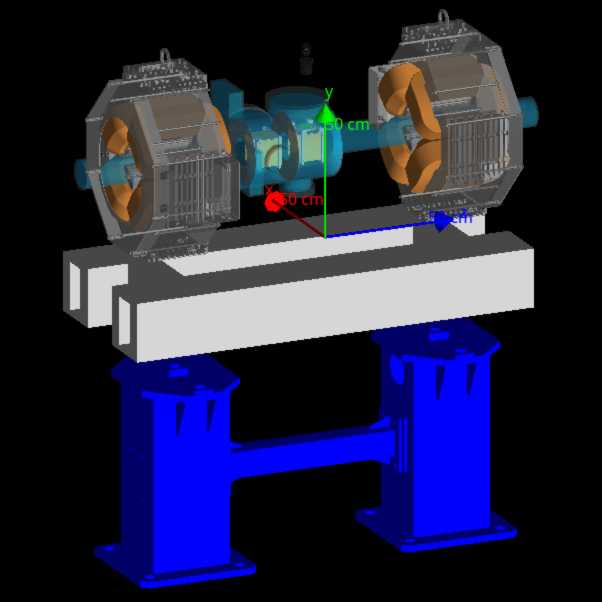
\includegraphics[width=\textwidth]{05_Conclusion/figures/fig000_geant4_sim2_a}
		\caption{The LWU and two quadrupoles.}
		\label{}
	\end{subfigure}
	~
	\begin{subfigure}[t]{0.615\textwidth}
		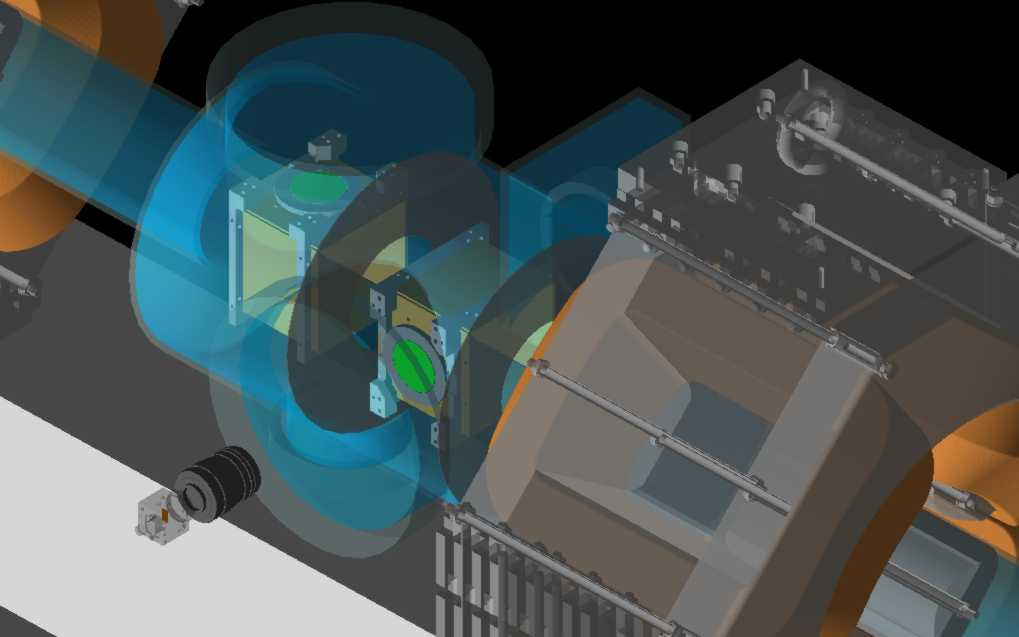
\includegraphics[width=\textwidth]{05_Conclusion/figures/fig000_geant4_sim2_b}
		\caption{Zoom on the two IPMs.}
		\label{}
	\end{subfigure}
	\caption[The geometry implemented in Geant4]{The geometry implemented in Geant4.}
	\label{chap5:fig:Geant4}
\end{figure}



% Florian: Je ne sais pas si il y a une échéance ? La production a plus ou moins déjà commencé
% All these aspects should be finalized by xxx (une date) allowing the production, installation and commissioning of the IPMS at ESS in xxx (autre date).

\subsection*{MCP calibration}
\addcontentsline{toc}{subsection}{MCP calibration}

\begin{wrapfigure}{l}{0.5\textwidth}
  \includegraphics[width=0.5\textwidth]{example-image-a}
	\caption[The calibration of the MCP is done with a VUV lamp]{The calibration of the MCP is done with a VUV lamp.}
	\label{chap5:fig:UV_calib}
\end{wrapfigure}

MCPs are mandatory to measure a profile with IPM in the ESS conditions. Unfortunately, these devices are sensitive to ageing effects. The gain will decrease over  time in the impacted areas by ions. Since the ESS beam will be stable in position, the MCP region in front of the beam will be more affected.

Therefore, at some point the profile measurement will be no longer reliable. To overcome this phenomenon it is necessary to calibrate the MCP regularly, i.e. perform a gain mapping and correct the profile by a software adjustment. This requires an uniform and stable source that routinely irradiates the MCP. The most common method relies on a VUV source \cite{Giacomini2011}. MCPs become sensitive to the photoelectric effect for wavelengths shorter than $200\,\mathrm{nm}$. The most basic VUV sources are deuterium discharge lamps that have broadband emission with a peaks at $160\,\mathrm{nm}$ \cite{HamamatsuUV,NewportUV}. It is also possible to generate VUV with excimer lasers or by using high order harmonic generation. Thermoionic emission was discarded due to the requirements imposed by the superconducting cavities. We are also considering the use of Electron Generator Arrays \cite{Satou2006, PhotonisEGA}. The calibration is currently being tested on the IPM test bench and Fig. \ref{chap5:fig:UV_calib} shows the principle of the experiment.

\subsection*{Remote acquisition system}
\addcontentsline{toc}{subsection}{Remote acquisition system}

In the case where the radiation background should shorten the MCP lifetime down to a year, it would be necessary to set a camera at remote distance in a shielded area. Two solutions are investigated to transport the image over up to $10\,\mathrm{m}$, where the camera can be shielded in the bottom of the nearby Stub. The solution to get a camera detecting single events, i.e. an ion hitting the MCP is been studied at ESS. The document presents two alternative imaging systems: the first one using a fiberscope and lenses is sketched on Fig. \ref{chap5:fig:schematic:1}, while the other one based on 2 mirrors and an objective lens can be seen on Fig. \ref{chap5:fig:schematic:2}.

\begin{figure}[!ht]
	\begin{subfigure}[t]{0.5\textwidth}
		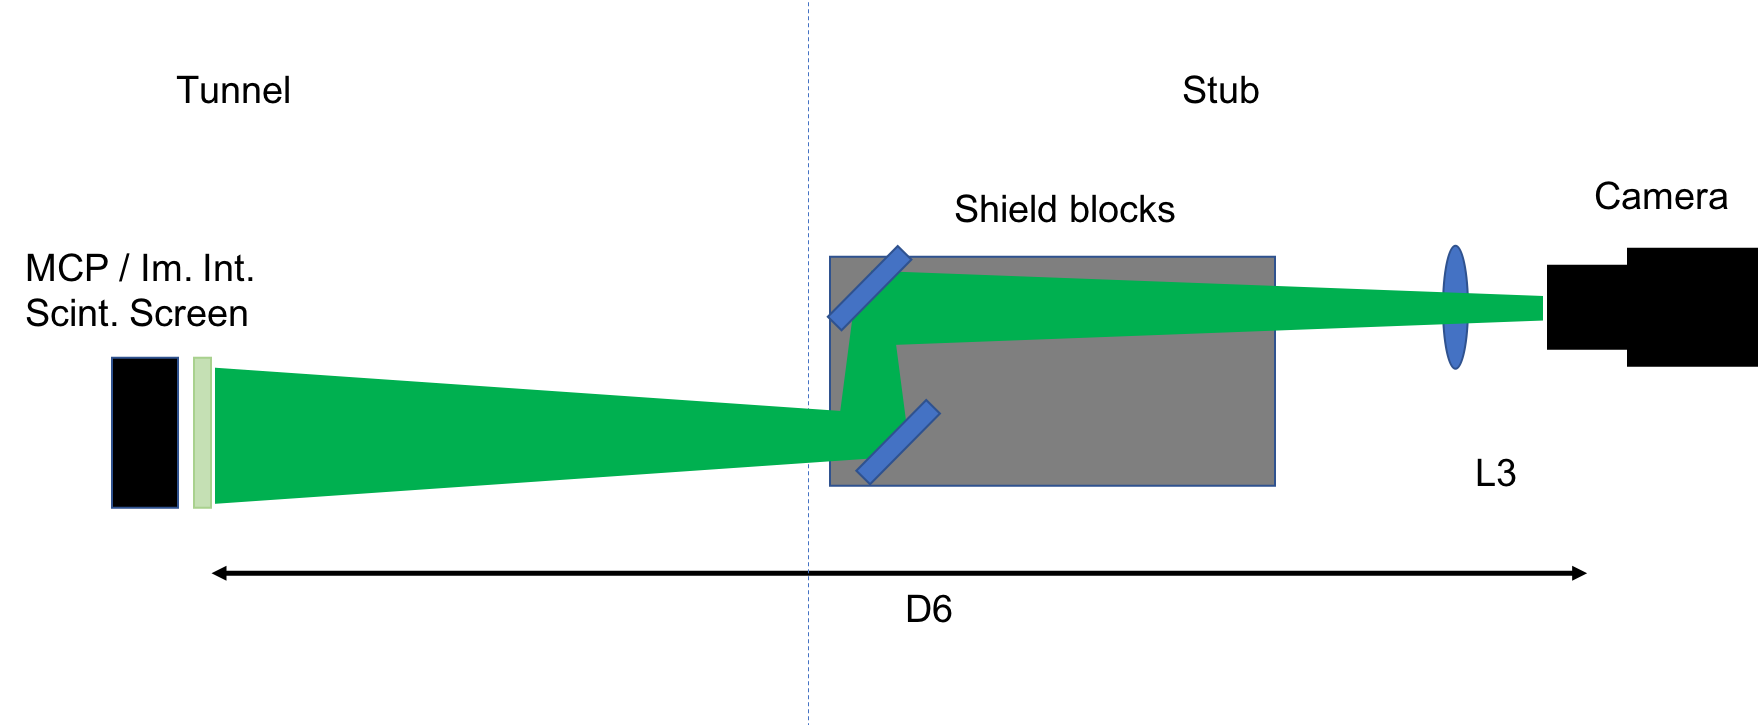
\includegraphics[width=\textwidth]{05_Conclusion/figures/fig000_schematic_telescop_lens}
		\caption{}
		\label{}
	\end{subfigure}
	~
	\begin{subfigure}[t]{0.5\textwidth}
		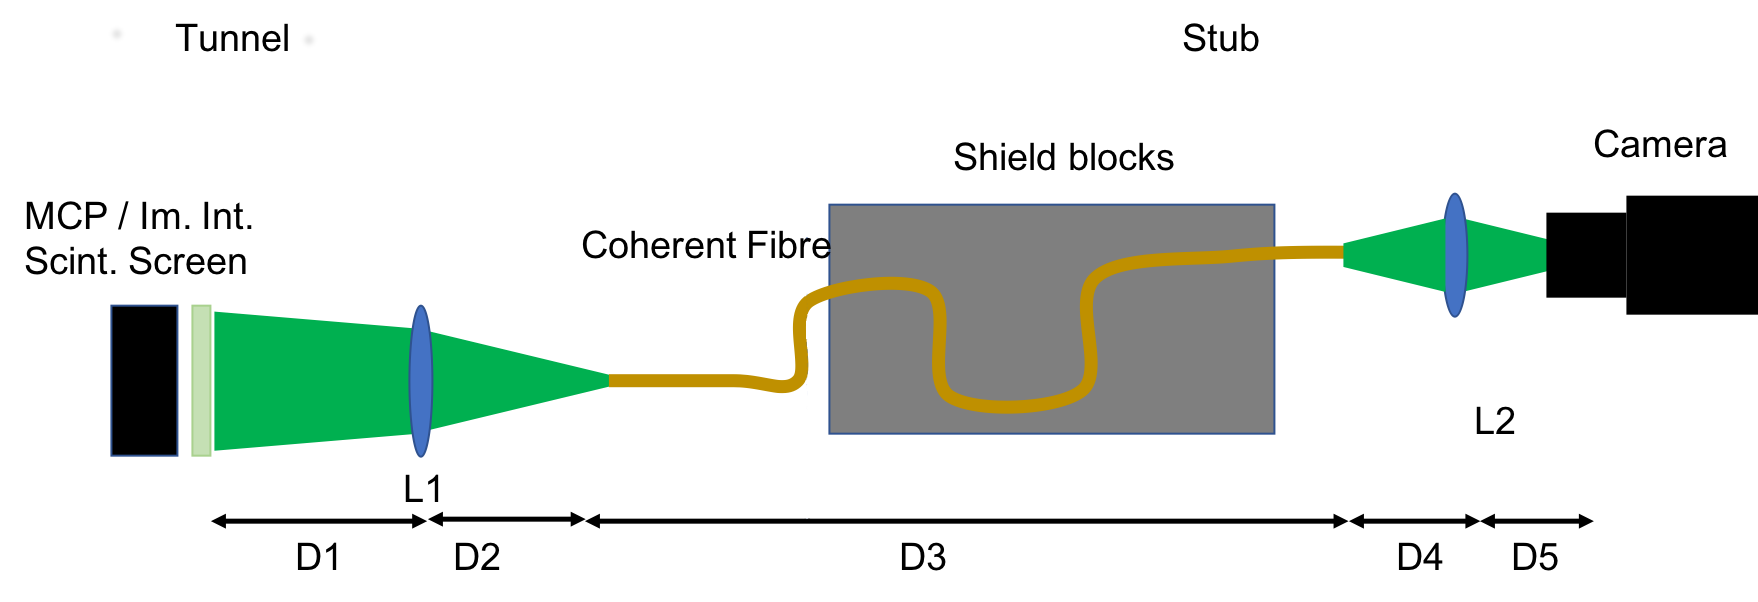
\includegraphics[width=\textwidth]{05_Conclusion/figures/fig000_schematic_coherentr_fiber}
		\caption{}
		\label{}
	\end{subfigure}
	\caption[]{}
	\label{chap5:schematic}
\end{figure}


Using a first order evaluation of the system transmission, one can start by selecting the focal lens required to make conjugate images. For the lens L1, the magnifications for the MCP is set, so as the geometrical aperture coupling light into the fibre.

The geometrical transmission for 0.5 numerical aperture of the fiberscope is about $3 \cdot 10^{-5}$ while it is a factor 4 below for the second system. Such an attenuation encourages to purchase stacked double MCP for increasing the output light.

The fiber attenuation is an important property to take into account. For instance, for silica fibers, this can be as low as a few $\mathrm{dB/km}$. We intent to use plastic coherent fibers. The material used is PMMA. This material is rather cheap, and it presents good optical quality and rather good transmission, typically $0.5\,\mathrm{dB/m}$ at $500\,\mathrm{nm}$. However, a full characterization of the system with the selected fiber will have to be done in order to prove and demonstrate the performance of the system. Lenses transmissions can be close to $100\,\mathrm{\%}$ with anti-reflection coating.

\subsection*{Final IPM design and production}
\addcontentsline{toc}{subsection}{Final IPM design and production}


% TODO: Finir
From the lessons learned with the prototypes, a final design of the IPM is on going\footnote{The design of final IPM has started, but is not frozen yet}, including few modifications from the prototype. This section presents briefly the new IPM design and its characteristics as well as the IPM production strategy. The differences between the prototypes and final IPMs are reported in Table \ref{chap5:tab:recap}. 

Preliminary simulations exhibit that the detection is possible if the readout system is enough sensitive. An important concern was about the choice of this readout. However without full characteristics of each system it is almost impossible to simulate the limits of detections. Therefore, these limits has been determined directly during beam tests. The tests clearly underline that the use of MCP is the best solution. Single stages MCP have been used during tests and they seems sufficient to detect profile at ESS. However IPMs will probably be ready before the accelerator reaches nominal conditions and double stage MCPs will allow profile measurements during the accelerator commissioning. The use of a double stage MCP reduces the maximal resolution achievable but this reduction is less important than the one induced by the remote acquisition system. The MCP with a strips readout provides the best performances in term of sensitivity and speed but needs a specifically designed readout electronics. Whereas an optical  MCP exposes decent performances with a high resolution and the acquisition relies only on \acrshort{cots} cameras. At the end the optical solution has been chosen. In any case the design of IPMs allows to easily upgrade the readout for future improvements thanks to the new mechanical design presented below.

Two field configurations were considered for the extraction field: asymmetric and symmetric. Simulations show that the symmetric setup provides a very good electric field uniformity even in longitudinal direction with simpler corrections. But asymmetric configuration also meets the requirements, and both case can be forseen at ESS since MCPs will be used. The electric field simulations have been verified with a relative comparison between the two cases and a good agreement has been observed. In practice, the symmetric configuration reduces the maximum potential to apply on each electrode reducing the need of HV feedtroughts above $20\,\mathrm{kV}$. These feedtroughs are complex, big and fragile increasing the complexity of the design. On the other hand, the number of HV power supplies, required in symmetric, mode is higher. Therefore the design is more expensive. For the final IPM, a $\pm\,15\,\mathrm{kV}$ symmetric configuration is forseen.

Space charge simulations point out that the measurement should be performed with ions at ESS. The in-house model has been checked during beam tests with the IPHI parameters. According to simulations, an electric field value of $2$ to $3\,\mathrm{kV/cm}$ seems enough and the final IPM design will target these electric field ranges. However it was not possible to reach stricly the same ESS bunch configuration. During the beam tests, the prototypes were not able to measure in electron mode whereas prototypes in ion mode were working fine. This strengthens the choice of ions for the profile measurement.

\begin{table}[!h]
  \centering
  \caption[Summary of differences between the prototype design and the final design]{Summary of differences between the prototype design and the final design.}
  \label{chap5:tab:recap}
  \begin{tabularx}{\linewidth}{lXX}
    \toprule
              & Prototype                                    & Final design            \\
    \midrule
    Amplifier & Single stage MCP                             & Double stage MCP        \\
    Readout   & Strips or phosphorus screens                 & Phosphorus screen (P43) \\
    Polarity  & Symmetric or asymmetric                      & Symmetric               \\
    Particle  & Ions or $e^{-}$                              & Ions                    \\
    Voltage   & $\pm 10\,\mathrm{kV}$ or $0/30\,\mathrm{kV}$ & $\pm 15\,\mathrm{kV}$   \\
    \bottomrule
  \end{tabularx}
\end{table}

The final IPMs will be produced following the ESS requirements for the superconducting cavities meaning that the IPMs will be assembled within an ISO-5 clean room environment.

During the tests at IPHI, we used a simple CF200 flange to support the IPM (Fig. \ref{chap4:IPM_photo2}). For the manufacturing of the IPM, we thought that two independent flanges CF200 and CF160 (Fig. \ref{chap5:fig:bride_double}) will ease the assembling process and the maintenance in clean room environment. This later configuration presents different advantages.

\begin{figure}[!ht]
	\begin{subfigure}[t]{0.25\textwidth}
		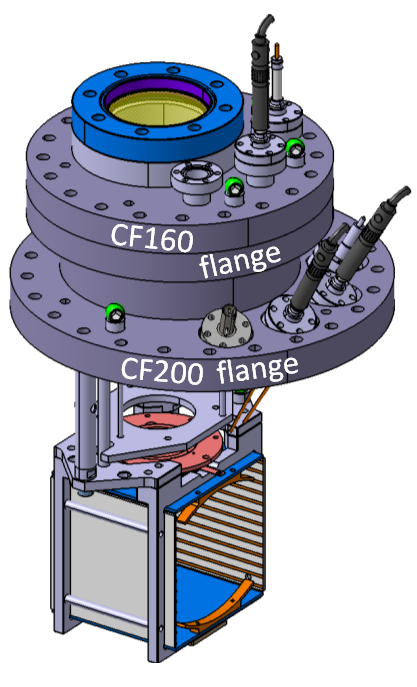
\includegraphics[width=\textwidth]{05_Conclusion/figures/fig000_bride_double2_a}
		\caption{A 3D drawing of the new design.}
		\label{}
	\end{subfigure}
	~
	\begin{subfigure}[t]{0.75\textwidth}
		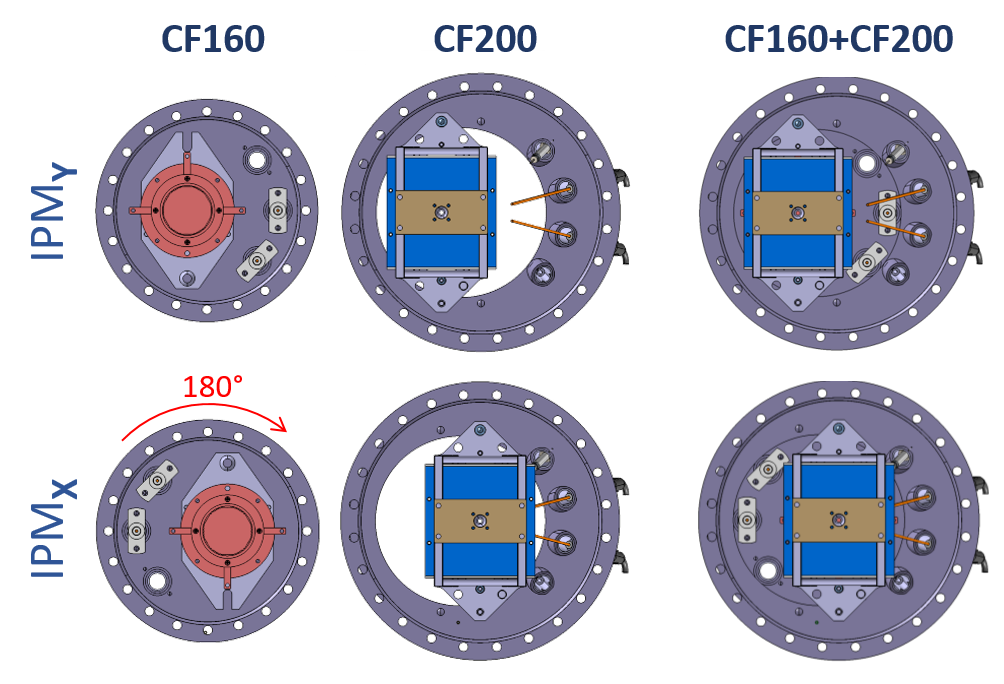
\includegraphics[width=\textwidth]{05_Conclusion/figures/fig000_bride_double2_b}
		\caption{The new design allow to remove MCP easily and is independent to the IPM direction.}
		\label{}
	\end{subfigure}
	\caption[The new IPM design]{The new IPM design \cite{JacquesCDR2019}.}
	\label{chap5:fig:bride_double}
\end{figure}

Once the complete IPM set is mounted on the LWU, alignment can be done by measuring all sight pods on the CF200. Then, if the MCP has to be removed (unscrew the CF160), the IPM cage linked to the CF200 stays fixed. The MCP can be changed but no alignment is necessary. This new configuration is compliant with a better reliability of the IPM since the MCP change may be done quickly, with no impact on alignment. The IPMs X and Y are similar: while X is centered on the CF200 LWU viewport, Y is shifted by $36\,\mathrm{mm}$ to its CF200 axis. The trick for mounting both IPMs, is to rotate the CF160 by $180°$ with respect to the CF200 flange. This is of great interest for manufacturing purposes.

For assembling the whole IPM, it is more convenient to prepare first the CF200 and all its belonging items, and then the CF160 ones. It allows minimizing the MCP in oxygen atmosphere. Furthermore, the set made of CF160 and MCP holder is light with a small lever arm easy to manipulate.

The IPMs will be delivered by pair and the first pairs are expected to be delivered to ESS at the middle of 2020.

Let's finish this manuscript from a perspective that goes beyond the ESS project. IPHI is a unique machine due to its powerful injector, but it has suffered delays in the past due to unfortunate circumstances. Over the last three years, a new dynamic is underway to fully exploit the accelerator capabilities. Today, IPHI is the first step of a new national compact neutron source: SONATE \cite{Marchix_2018}. As stated in the first chapter, the LLB is closing its last research reactors this year. Some estimates show that the availability of neutrons at the national level will fall by more than $90\,\mathrm{\%}$ within the next 10 years.

During the tests, the versatility of IPHI greatly helped to characterize the IPMs. However, some tests were limited by a lack of beam information during operation. Indeed, only two types of diagnosis were available: BPMs and BCMs. IPMs are a very interesting solution for IPHI because they measure the size and  the position in a non-intrusive way. A close collaboration has started in order to provide to IPHI an IPM system that fulfills the present and future needs. This new project will greatly benefit from the studies and experiences presented in this thesis.

\cleardoublepage
\section*{Bibliography}
\addcontentsline{toc}{section}{Bibliography}
\label{ch2:bib}
\printbibliography[heading=subbibliography]

%%%%% 
%Firstly, we discovered that one of the pMCP was broken and finally decided to change it.

%After more than 2 weeks, we did not have seen a beam profile. We finally succeeded after working thoroughly with a beam dynamic physicist, scanning the beam as well as the deviation dipole, the correction steerers and the quadruples. We effectively got a nice transverse profile, completely correlated to the beam location and intensity, but having a strange behavior. Indeed, the pulse presented a position oscillation, starting to move in one direction, and coming back after $5$-$7$ seconds to its initial position, and so on! It was similar to an insulator, starting to accumulate electric charges and releasing them suddenly… We inquired on our IPM which are designed with insulators (Peeks, Macor, ceramics), since we did not find anything strange on the beam side. It lasted several days with any explanation, until a physicist gets to work on a BPM, to discover a very impressive correlation between the BPM and the IPM beam coordinates! Up to now, IPHI has not a real explanation for this behavior. This event sounds like a big relief and gave us a better confidence in our measurements.

%  Later on, we discovered that the beam presents also 2 components as shown in the manuscript: a mix of a core and narrow beam at high beam intensity and a large component at low intensity.
%  We have also encountered some difficulties to make systematic studies because it is not easy to reproduce a beam condition, even with previously beam parameters. Nevertheless, it was useful to have such versatile facility where we were able to regain the expected MCP behaviors. Many measurements were done as shown in the thesis, allowing investigating many parameters and for preparing the second beam tests on September 2018. The goal will be to focus on the profile measurement feasibility in nominal conditions, in ion mode since simulations have already shown that electron detection is hopeless.

%  During this last campaign, we finally work in such beam conditions, which are even worse than the ESS ones. These relevant results are summarized in the Table \ref{chap4:extrapolationMCP} demonstrating that we should be able to measure beam profile at ESS at nominal conditions, for each pulse beam.

%%
% In this manuscript I presented a large part of the work done on the study, design and testing of non-invasive profilers based on ionization. This chapter describes the tasks currently underway or in perspective for the conception of the final diagnostics and summarize the previous chapters. 

% The MCP is 40\,mm diameter and the fiber diameter is 2\,mm. The geometrical transmission T of the lens to the fiber is defined by the aperture of the lens, called the F-number or F\#, the focal lens, F and the distance between the screen and the lens, D1:
% \begin{equation}
%  T=\frac{1}{2} \left(1 - cos\left(\theta\right)\right)
% \end{equation}
% with $\theta = \rm arctan\left (\frac{F/F\#}{2D} \right )$

% Unfortunately, the information about the background particles was finally given after the beginning of the writing phase of this thesis. Nevertheless, the simulation base is implemented and I hope that this work will continue and lead to results that may provide additional knowledge.
% \section*{Conclusion}
% \addcontentsline{toc}{section}{Conclusion}

% \subsection*{The ESS linac and IPM}
% \addcontentsline{toc}{subsection}{The ESS linac and IPM}

% Intense neutron sources are very difficult to achieve. Historically, nuclear reactors have been widely used as intense neutron sources. In Europe the situation is quite critical because most of research reactors will close within the next decade. In that context, the European Spallation Source is being built close to Lund, in Sweden. ESS will push back the limits of existing spallation sources by means of an high end powerful linear accelerator. To ensure the safety of the machine during the commissioning and operations, many diagnostics are foreseen along the accelerator.

% This thesis described the design of one of these diagnostics: the Ionization Profile Monitor(IPM). IPMs are based on the ionization of residual gas. This is one of the most effective methods, but it is nevertheless quite complex to implement. The first IPMs date back to the 1960s but the method has been improved significantly with advances in detector, electronics and computer sciences. The IPM method is now mature and used in several installations. In this thesis, the existing methods have been reviewed in order to find the best solution that may match with the ESS requirement. This have been done by simulations first and, in a second time, by building and testing prototypes.

% \subsection*{IPM feasibility}
% \addcontentsline{toc}{subsection}{IPM feasibility}

% Three key points had been identified: number of primary particles, distortion effects of the profile, the choice of the reading system.

% The conditions at ESS are particularly unfavorable for the ionization cross sections and the high vacuum in the accelerator does not work in our favour. Calculations (Bethe and PAI) and simulations show that the order of magnitude of the number of primary particles is about a few thousand particles per pulse beam under nominal ESS conditions. This number seems sufficient to carry out a measurement assuming that tey are correctly detected.

% Non-uniformities of the electric field can be effectively corrected using field correctors and separation discs regardless of the power supply configuration used. However, the symmetrical mode is easier to correct and reduces the maximum voltage level required.
% Simulations clearly show that ions are less sensitive to the space charge effect and initial velocity of particle. Measurement with electrons introduces an error that does not allow the ESS requirements to be met. It is impossible to install a corrector magnet to constrain the electron trajectories. Therefore, the profile measurement will be done with ions.

% The use of ions makes the choice of the readout a more complicated. Strips are an robust method but require enough sensitive and low-noise electronics to be able to detect such low charge quantities.
% The MCPs amplifies the signal but these devices tend to age. Silicon detectors look very promising because they are very sensitive, resistant and fast. However, the detection of low energetic ions is not ensured and the implementation is quite complex.

% \subsection*{Prototype design and tests}
% \addcontentsline{toc}{subsection}{Prototype design and tests}

% First, the feasibility of silicon detectors was verified on the
% At IRMA ion implanter, the feasibility of silicon detectors was checked.
% The detection seams possible but with almost no error margin. We also observed that the silicon sensor was quickly damaged by the incident ions. Therefore, we discarded this readout for ESS usage.

% Then, a complete IPM testing platform has been developed in order to test the two remaining readouts. The IPM prototypes have been designed to be totally independent to the readout. Therefore the testing platform was quite versatile.

% The prototype been tested at IPHI, a $3\,\mathrm{MeV}$ proton accelerator. A complete characterization of the two IPMs was done. Good agreements have been found between the two types of IPMs and existing IPHI diagnostic. The tests were also a kind a commissioning of the machine confirming that the IPMs is a great tool to tune a beam. According to results the measurement seams possible at ESS with even a single stage MCP. The results has been presented to ESS collaborators during a Critical Design Review.

% The final IPM will use double stages MCP polarized in symmetric HV configuration. The symmetric setup provides really good uniformity with basic corrections. It also reduces the maximum potential to apply to electrode.
% A MCP with strips may provides best performances in term of sensitivity and speed. But a complicated readout electronic must be designed for that purpose. Whereas a MCP optical exposes decent performances and an high resolution but the acquisition relies only on COTS cameras.
% At the end the optical solution was chosen. Anyway the design of IPMs allows to easily upgrade the readout for future improvements.

% The double stage MCP will allow measurement during the accelerator commissioning. Therefore may be ready even before than the accelerator reaches its nominal conditions. On the other hand the use of an double stage MCP reduces the maximal resolution but this reduction is less important compare to the one induced by the remote acquisition system

% The final IPMs will be produced following the ESS requirement for the superconducting cavities. This means that the IPMs will be assembled within an ISO-5 clean room environnement. The IPMs will be delivered by pair and the first pairs is expected to be delivered to ESS in the beginning of 2020.

%\subsection{Personal conclusion}

%\end{refsection}
